Organizator spotkań jest komponentem wspierającym zarządzanie tym typem obiektów. 
Pozwala na wgląd w listę wszystkich spotkań na 4 rożne sposoby:
\begin{itemize}
	\item widok w kontekście wybranego dnia,
	\item widok w kontekście wybranego tygodnia,
	\item widok w kontekście wybranego miesiąca,
	\item widok tabelaryczny wszystkich spotkań.
\end{itemize}

\begin{figure}[H]
	\centering
	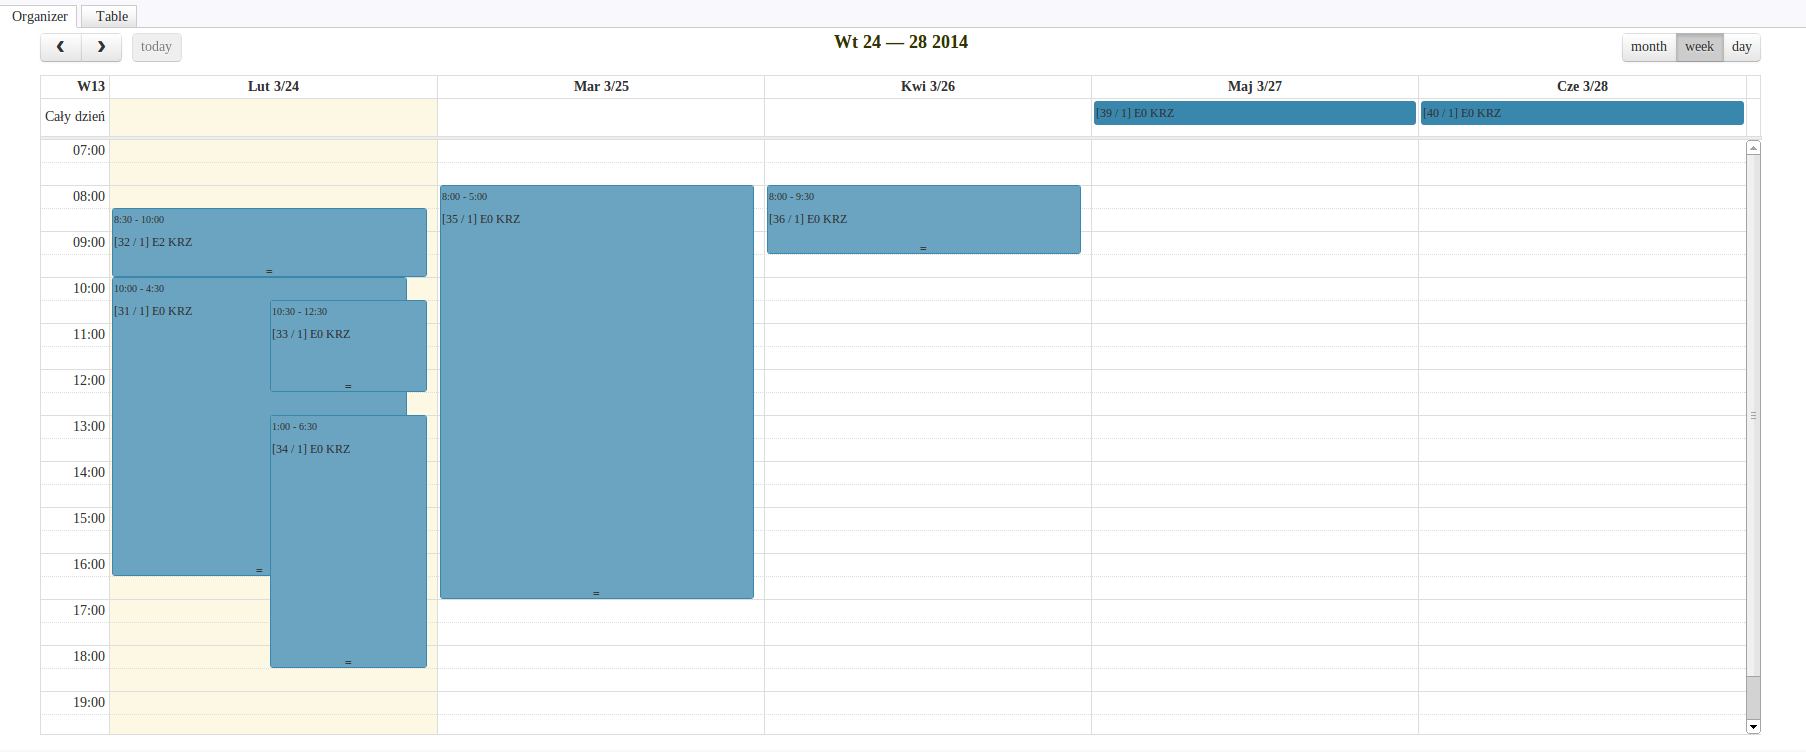
\includegraphics[width=1.0\textwidth]{images/calendarComponent-organizer}
	\caption[Komponent kalendarza wspierający organizację spotkań - organizer]{
		Komponent kalendarza wspierający organizację spotkań - organizer, źródło: opracowanie własne			
	}
	\label{app:component_calendar_organizer}
\end{figure}
\begin{figure}[H]
	\centering
	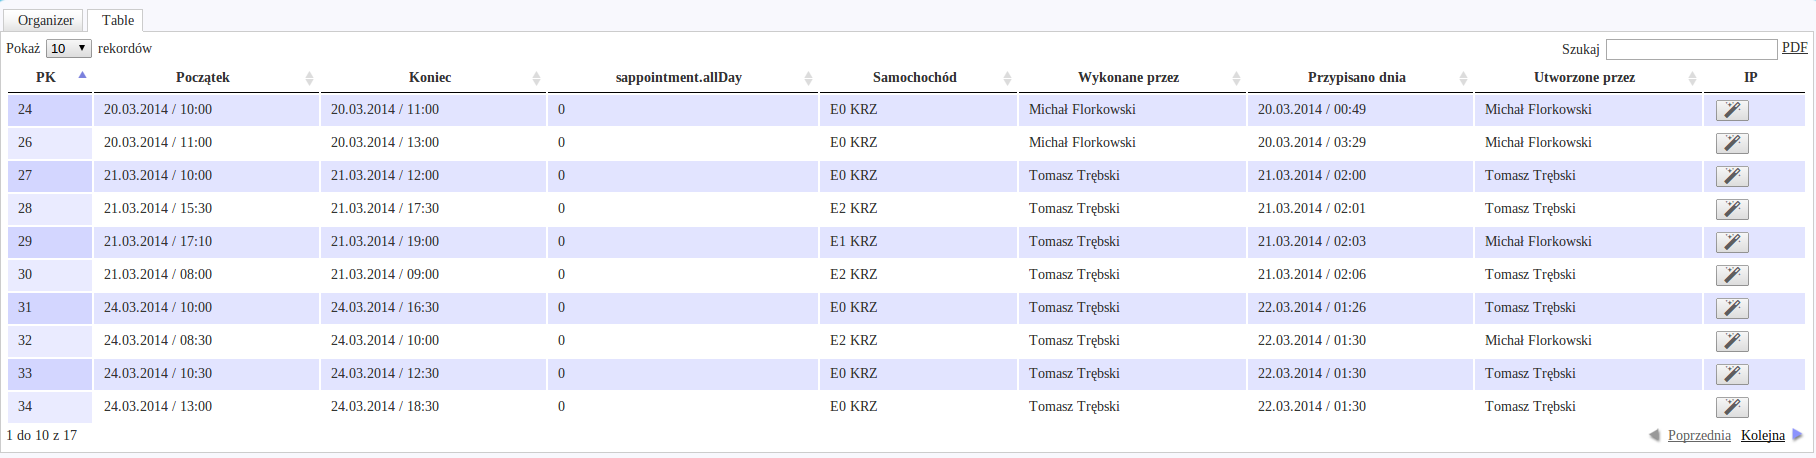
\includegraphics[width=1.0\textwidth]{images/calendarComponent-table}
	\caption[Komponent kalendarza wspierający organizację spotkań - tabela]{
		Komponent kalendarza wspierający organizację spotkań - tabela, źródło: opracowanie własne	
	}
	\label{app:component_calendar_table}
\end{figure}	

Z poziomu organizera możliwe jest natomiast otwieranie strony domenowej dla wybranego spotkania, dostarczającej znacznie więcej informacji niż sam organizator oraz uruchomienie przewodnika utworzenia nowego spotkania. Ważną cechą tego przewodnika jest to, że zakres dat wybrany w organizatorze jest zachowany. Sam kreator został napisany w oparciu o technologię \textbf{Spring Web Flow}, dzięki czemu na poziomie jednego komponentu można wprowadzić dane takie jak: 
\begin{itemize}
	\item mechanik, który będzie odpowiedzialny za wizytę,
	\item mechanik raportujący dane spotkanie, niemniej taką możliwość posiadają jedynie osoby uprawnione do tego,
	\item wybrany samochód,
	\item lista zadań do wykonania podczas wizyty,
	\item opcjonalny komentarz dla wizyty.
\end{itemize}